\subsection{Comparison to World Data and SAID Fits}\label{sec:results.conclusion}
This section will discuss comparisons of our data with SAID fits and the \abbr{GPD} handbag model. The SAID parameterization, discussed in~\cite{SAID}, for this analysis was based upon previous data observables in conjunction with the new cross-section measurement presented in this analysis.

\subsubsection{Differential Cross-Sections $\frac{\lowercase{d}\sigma}{\lowercase{d}\Omega}$}\label{diffXsection}
The differential cross-sections $\frac{\lowercase{d}\sigma}{\lowercase{d}\Omega}$ are illustrated in Figs.~\ref{fig:results.xsection1},~\ref{fig:results.xsection2},~\ref{fig:results.xsection3},~\ref{fig:results.xsection4}. A brief discussion is presented in Sec.~\ref{sec:discussion}.
\begin{figure}[h!]\begin{center}
\includegraphics[width=\figwidth,height=1.25 \hfigheight]{\figures/analysis/kk01a.pdf}%angle=90,
\caption[The $\pi^0$ proton photoproduction cross section, $(d\sigma/d\Omega)$, at $E_{\gamma}$ = 1.275 -- 2.225~GeV versus $\cos\theta$ where $\theta$ is the pion center-of-mass production angle]{\label{fig:results.xsection1}(Color online) The $\pi^0$ proton photoproduction cross section, $(d\sigma/d\Omega)$, at $E_{\gamma}$ = 1.275 -- 2.225~GeV versus $\cos\theta$ where $\theta$ is the pion center-of-mass production angle. Photon energy is indicated by $E$, while the center-of-mass total energy is indicated by $W$. Red solid (blue solid) lines show the SAID KU14 (DU13~\protect\cite{Dugger13}) calculations. Black solid lines give the BG2011-02 BnGa~\protect\cite{BonnGat}) predictions. Experimental data are from the current measurement (red filled circles), CLAS~\protect\cite{Dugger07} (black filled circles), GRAAL~\protect\cite{Graal} (magenta open circles), LEPS~\protect\cite{LEPS} (blue plus), CB-ELSA~\protect\cite{ELSA05}~\cite{ELSA11} (green crosses) and previous bremsstrahlung measurements~\protect\cite{brem} (black open circles). Plotted uncertainties are statistical. The plotted points from previously published experimental data are those data points within $\pm$3~MeV of the photon energy indicated on each panel.}
\end{center}\end{figure} 

\begin{figure}[h!]\begin{center}
\includegraphics[angle=90,width=\figwidth,height=1.5 \hfigheight]{\figures/analysis/kk02a.pdf}
\caption[The $\pi^0$ proton photoproduction cross section at $E_{\gamma}$ = 2.275 -- 3.375~GeV versus cosine of the pion center-of-mass production angle]{\label{fig:results.xsection2}(Color online) The $\pi^0$ proton photoproduction cross section at $E_{\gamma}$ = 2.275 -- 3.375~GeV versus cosine of the pion center-of-mass production angle. Notation as in Fig.~\protect\ref{fig:results.xsection1}.}
\end{center}\end{figure}

\begin{figure}[h!]\begin{center}
\includegraphics[angle=90,width=\figwidth,height=1.5 \hfigheight]{\figures/analysis/kk03a.pdf}
\caption[The $\pi^0$ proton photoproduction cross section at $E_{\gamma}$ = 3.425 -- 4.425~GeV versus cosine of the pion center-of-mass production angle]{\label{fig:results.xsection3}(Color online) The $\pi^0$ proton photoproduction cross section at $E_{\gamma}$ = 3.425 -- 4.425~GeV versus cosine of the pion center-of-mass production angle. Notation as in Fig.~\protect\ref{fig:results.xsection1}.}
\end{center}\end{figure}

\begin{figure}[h!]\begin{center}
\includegraphics[angle=90,width=\figwidth,height=1.5 \hfigheight]{\figures/analysis/kk04a.pdf}
\caption[The $\pi^0$ proton photoproduction cross section at $E_{\gamma}$ = 4.475 -- 5.425~GeV versus cosine of the pion center-of-mass production angle]{\label{fig:results.xsection4}(Color online) The $\pi^0$ proton photoproduction cross section at $E_{\gamma}$ = 4.475 -- 5.425~GeV versus cosine of the pion center-of-mass production angle. Notation as in Fig.~\protect\ref{fig:results.xsection1}.}
\end{center}\end{figure}
\FloatBarrier
\subsubsection{Excitation Functions}
\label{ExtFun}
The excitation functions $\frac{\lowercase{d}\sigma}{\lowercase{d}\Omega}$ at fixed $\theta$ are illustrated in Figs.~\ref{fig:wdist},~\ref{fig:wdist2}. A brief discussion is written in Sec.~\ref{sec:discussion}.
\begin{figure}[h!]\begin{center}
\includegraphics[width=\figwidth,height= \hfigheight]{\figures/analysis/DSG/mm01a-eps-converted-to.pdf}
\caption[Fixed angle excitation functions of the $\pi^0$ photoproduction cross section, $(d\sigma/d\Omega)$, off the proton at $\theta$ = 31 -- 75$^\circ$ versus center-of-mass total energy $W$]{\label{fig:wdist}(Color online) Fixed angle excitation functions of the $\pi^0$ photoproduction cross section, $(d\sigma/d\Omega)$, off the proton at $\theta$ = 31 -- 75$^\circ$ versus center-of-mass total energy $W$. The pion center-of-mass production angle is shown. Plotted uncertainties are statistical. The plotted points from previously published experimental data are those data points within $\pm$2$^\circ$ of pion center-of-mass production angle indicated on each panel. Notation as in Fig.~\protect\ref{fig:results.xsection1}.}
\end{center}\end{figure}


\begin{figure}[h!]\begin{center}
\includegraphics[width=\figwidth,height= \hfigheight]{\figures/analysis/DSG/mm02a-eps-converted-to.pdf}
\caption[Fixed angle excitation functions of the $\pi^0$ photoproduction cross section, $(d\sigma/d\Omega)$, off the proton at $\theta$ = 76 -- 140$^\circ$ versus center-of-mass total energy $W$]{\label{fig:wdist2}(Color online) Fixed angle excitation functions of the $\pi^0$ photoproduction cross section, $(d\sigma/d\Omega)$, off the proton at $\theta$ = 76 -- 140$^\circ$ versus center-of-mass total energy $W$. Notation as in Fig.~\protect\ref{fig:results.xsection1}.}
\end{center}\end{figure}


\FloatBarrier
\clearpage
\subsubsection{$t$-Dependence}
\label{tDep}
The $t$-dependence of $\frac{\lowercase{d}\sigma}{\lowercase{d}t}$ at fixed $E_{\gamma}$ are illustrated in Figs.~\ref{fig:t_data},~\ref{fig:t_data2},~\ref{fig:t_data3},~\ref{fig:t_data4}. A brief discussion is written in Sec.~\ref{sec:discussion}.
\begin{figure*}[htb!]
\includegraphics[width=\figwidth,height= \hfigheight]{\figures/analysis/DSG/kk01b-eps-converted-to.pdf}
\caption[$\pi^0$ photoproduction cross section, $(d\sigma/dt)$, off the proton at $E_{\gamma}$ = 1275 -- 2225~MeV versus momentum transfer $t$]{\label{fig:t_data}(Color online) $\pi^0$ photoproduction cross section, $(d\sigma/dt)$, off the proton at $E_{\gamma}$ = 1275 -- 2225~MeV versus momentum transfer $t$. Notation as in Fig.~\protect\ref{fig:results.xsection1}.}
\end{figure*}

\begin{figure*}[htb!]
\includegraphics[angle=90,width=\figwidth,height= \hfigheight]{\figures/analysis/DSG/kk02b-eps-converted-to.pdf}
\caption[$\pi^0$ photoproduction cross section, $(d\sigma/dt)$, off the proton at $E_{\gamma}$ = 2275 -- 3375~MeV versus momentum transfer $t$]{\label{fig:t_data2}(Color online) $\pi^0$ photoproduction cross section, $(d\sigma/dt)$, off the proton at $E_{\gamma}$ = 2275 -- 3375~MeV versus momentum transfer $t$. Notation as in Fig.~\protect\ref{fig:results.xsection1}.}
\end{figure*}

\begin{figure*}[htb!]
\includegraphics[angle=90,width=\figwidth,height= \hfigheight]{\figures/analysis/DSG/kk03b-eps-converted-to.pdf}
\caption[$\pi^0$ photoproduction cross section, $(d\sigma/dt)$, off the proton at $E_{\gamma}$ = 3425 -- 4425~MeV versus momentum transfer $t$]{\label{fig:t_data3}(Color online) $\pi^0$ photoproduction cross section, $(d\sigma/dt)$, off the proton at $E_{\gamma}$ = 3425 -- 4425~MeV versus momentum transfer $t$. Notation as in Fig.~\protect\ref{fig:results.xsection1}.}
\end{figure*}

\begin{figure*}[htb!]
\includegraphics[width=\figwidth,height= \hfigheight]{\figures/analysis/DSG/kk04b-eps-converted-to.pdf}
\caption[$\pi^0$ photoproduction cross section, $(d\sigma/dt)$, off the proton at  $E_{\gamma}$ = 4475 -- 5425~MeV versus momentum transfer $t$]{\label{fig:t_data4}(Color online) $\pi^0$ photoproduction cross section, $(d\sigma/dt)$, off the proton at  $E_{\gamma}$ = 4475 -- 5425~MeV versus momentum transfer $t$. Notation as in Fig.~\protect\ref{fig:results.xsection1}.}
\end{figure*}

\begin{figure}[htpb]\begin{center}
		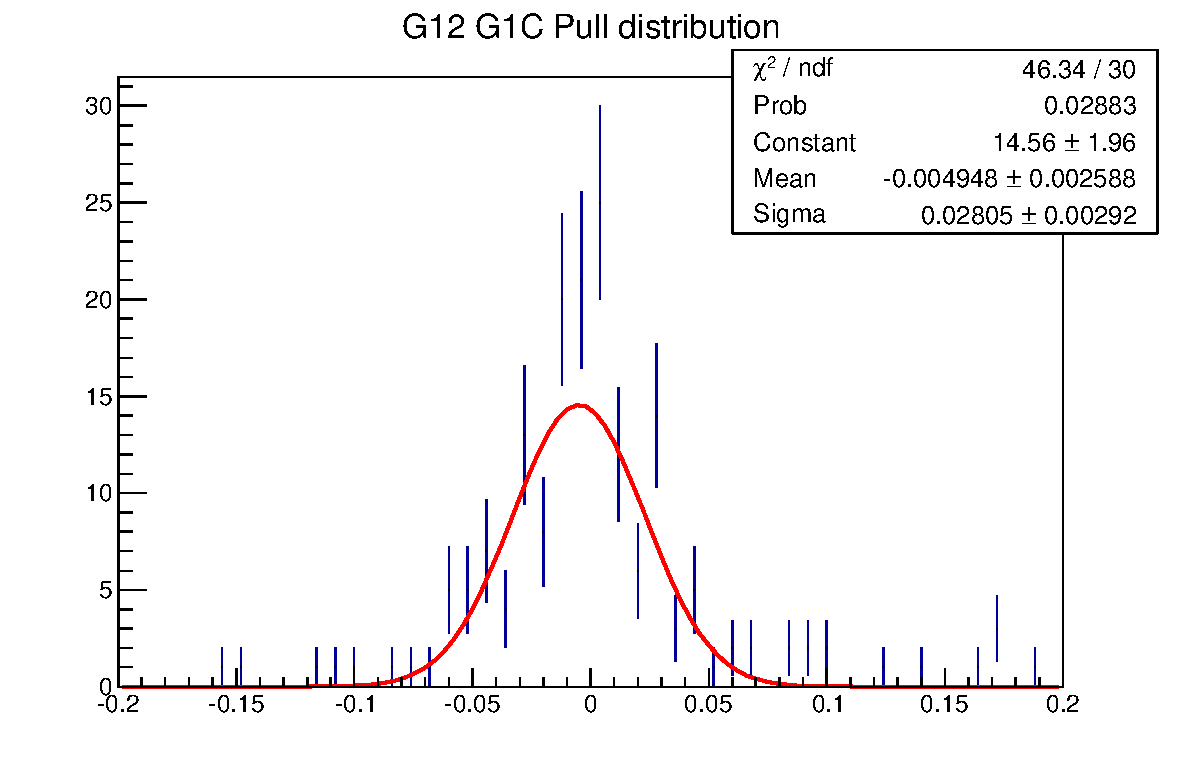
\includegraphics[width=0.7\columnwidth]{/Users/michaelkunkel/WORK/GIT_HUB/Pi0_Papers/ANALYSIS_NOTE/RESULTS/G12_Pi0_XSection_pull.pdf}
		\caption{\label{fig:pi0.xsec.pull}Pull distribution for g12/g1c comparison of data shown in Figs.~\ref{fig:results.xsection1} and \ref{fig:results.xsection2}.}
	\end{center}\end{figure}

\FloatBarrier
%\subsubsection{Improvement to Previous SAID Fits}
%\subsubsection{CGLN Amplitudes}
%To demonstrate the impact of our data on the global fit, in Fig.~\ref{fig:CGLN1} we show, the distribution of amplitudes (see Sec.\ref{sec:CGLN}) at one particular pion production angle $\Theta^{CM}_{\pi^0}=60^{\circ}$ as a function of $W$.
%The blue lines are results of the fit to world data and the red lines are solutions with our data included. The dashed lines are 
%for imaginary parts of amplitudes. For the real part of amplitudes the blue (dashed-dotted) lines are results of the fit to previous 
%data and red (solid) are results of the fit with our data included. Vertical arrows show positions of  $N^{*}$ resonances listed as 
%$4^*$-resonances in PDG. As one can see, the main features of previous solution are preserved, however the
%strength of different groups of resonances are affected and for some the contributions almost negligible, questioning their 
%overall existence. 
%
%Detailed amplitude analysis of the world data with the inclusion of our new data in entire kinematic range at all angles 
%and invariant masses available will allow to constrain positions, Breit-Wigner widths and couplings of different resonances 
%as well as dismiss and/or observe missing resonance states with high statistical confidence.
%
%\begin{figure}[!ht]
%  \centering
%  \subfloat[][]{\includegraphics[width=2.5in, height=2.5in, angle=90,valign=c]{\figures/analysis/FULL_AMPL/v4a-eps-converted-to.pdf}\label{fig:CGLN1_I}} \quad
%  \subfloat[][]{\includegraphics[width=2.5in, height=2.5in, angle=90,valign=c]{\figures/analysis/FULL_AMPL/v4b-eps-converted-to.pdf}\label{fig:CGLN1_II}} \\
%  \subfloat[][]{\includegraphics[width=2.5in, height=2.5in, angle=90,valign=c]{\figures/analysis/FULL_AMPL/v4c-eps-converted-to.pdf}\label{fig:CGLN1_III}} \quad
%  \subfloat[][]{\includegraphics[width=2.5in, height=2.5in, angle=90,valign=c]{\figures/analysis/FULL_AMPL/v4d-eps-converted-to.pdf}\label{fig:CGLN1_IV}}
%      \caption[CGLN amplitude at $\theta $= 60$^\circ$]{(Color online) CGLN amplitude~\protect\cite{CGLN}
%                at $\theta $= 60$^\circ$.  Vertical arrows indicate 
%		resonance energies W$_R$ (4$^\ast$-resonances)~\protect\cite{pdg2014}. 
%		Notation as in Fig.~\protect\ref{fig:results.xsection1}.}
%        \label{fig:CGLN1}
%\end{figure}

\FloatBarrier
\subsubsection{SAID $\chi^2$ Improvements}\label{sec:chi}
The measured cross-section presented in this analysis yielded an improvement to the SAID fit. This improvement, in the form of a $\chi^2/dp$, can be seen in Fig.~\ref{fig:chi_sq}, where the new cross-section measurement is depicted in red while the previous is depicted in blue. Decreasing the $\chi^2/dp$ reflects the ``goodness" of fit and overall quality of fitting the data. This is important because if a fit determines a resonance or change in amplitude, the quality of the fit determines the accuracy of the solution.  
\begin{figure}[h!]\begin{center}
\includegraphics[width=\figwidth,height= \hfigheight]{\figures/analysis/dsg1a-eps-converted-to.pdf}
\caption[Energy dependence of the $\chi^2/dp$ comparison to previous SAID fits]{\label{fig:chi_sq}Energy dependence of the $\chi^2/dp$ comparison to previous SAID fits. Blue points depict previous DU13 solution, while the red points depict the new KU14 solution.}
\end{center}\end{figure} 
\FloatBarrier
%
%
\subsubsection{Discussion of SAID Fits and Comaprision to World Data}\label{sec:discussion}
This measurement agrees with existing world data at low energy where there are numerous previous measurements. At higher energies there appears to be partial disagreement with~\cite{brem} from which this data were taken from the untagged bremsstrahlung beam. This disagreement can be seen in some of the low angle $\theta$ excitation functions in Sec.~\ref{ExtFun}. However, with the same data presented in~\cite{brem} there is agreement, noticeably at angles $\theta = 89^\circ$ and $\theta = 92^\circ$. Since the excitation function measurements performed in this analysis agree well in the low energy domain and also the data is congruent throughout the $\theta$ spectrum, further investigation is needed into the method of~\cite{brem} to understand where or why the discrepancy exists.
%
%
\FloatBarrier
%\subsubsection{Comparison with Theory}\label{Kroll}
%The handbag model calculations by Kroll \textit{et al.}~\cite{Huang2000} does not agree with the present data as seen in Fig.~\ref{fig:kroll}. There is no supporting material to explain why this model does not work well. Future models using Regge-parametrization are currently being formulated independently of this analysis. These high energy \pizT cross-sections will be the basis for all future models.
%\begin{figure}[h!]\begin{center}
%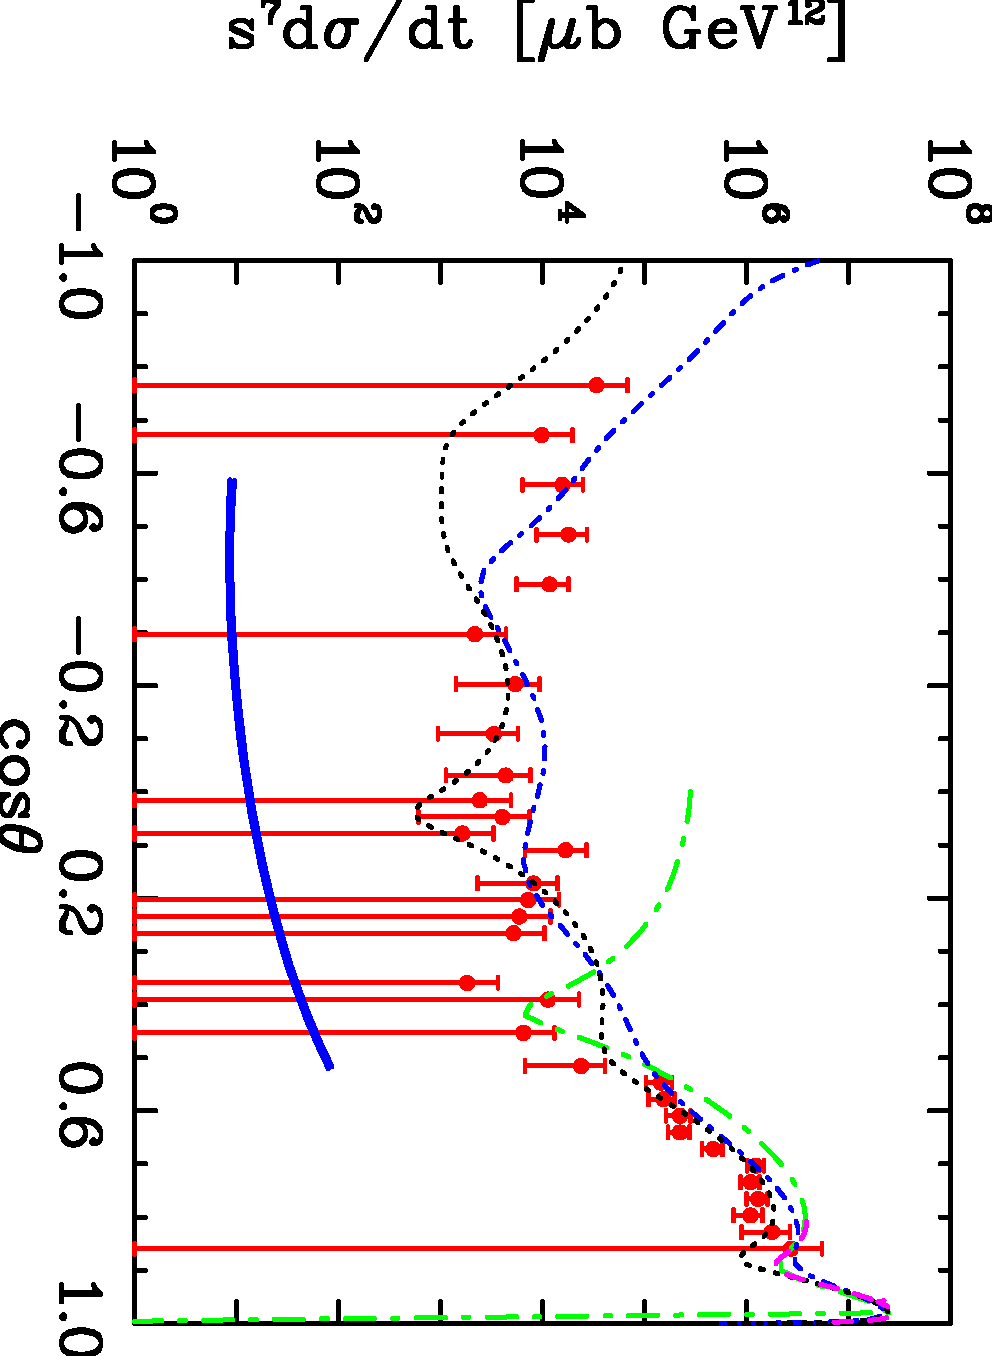
\includegraphics[width=\figwidth,height= \hfigheight]{\figures/analysis/DSG/kroll-eps-converted-to.pdf}
%\caption[Comparison of the $\pi^0$ differential cross section  photoproduction data to \abbr{GDP} handbag model]{\label{fig:kroll}Comparison of the $\pi^0$ differential cross section  photoproduction data to \abbr{GDP} handbag model. Experimental data at $s$ = 11.08~GeV$^2$ are from the current (red filled circles). The theoretical prediction at $s$ = 10~GeV$^2$ by Kroll \textit{et al.}~\protect\cite{Huang2000} is given by blue solid line.}
%\end{center}\end{figure} 
%\FloatBarrier

\section{Conclusions}
This manuscript explained the procedure of collecting data in the \abbr{CLAS} detector for the g12 experiment. Data corrections, kinematic fitting and fiducial cuts were used to clean the data to the order of $\approx$98\% signal. Differential cross-sections in two representation, $\frac{d\sigma}{d\Omega}$ and $\frac{d\sigma}{dt}$, were given along with comparisons to the existing world data, comparison existing Bonn-Gatchina fits and new SAID parameterization fits. The cross-sections measured in this analysis agreed well with the existing world data for low incident beam energies, while there was a slight discrepancy with the previous limited high energy cross-sections. The fits using the SAID parametrization yielded a $\chi^2/dp$ lower than previous existing fits. The data set explained in this analysis is now 10\% of the world data for \pizT photoproduction. More development of theory is need to properly explain \pizT production at incident photon beam energies higher than 2.8~GeV.





 